\documentclass[twocolumn,10pt]{article}
\usepackage{url,graphicx,tabularx,array}%,geometry} %,fullpage,amsfonts,amsmath}
\usepackage{amsmath,amsthm,amsfonts,amssymb,amscd,mathabx,ulem}
\usepackage{fullpage}
\usepackage{lastpage}
\usepackage{enumerate}
\usepackage{fancyhdr}
\usepackage{mathrsfs}
\usepackage[margin=1.5cm]{geometry}
\usepackage{listings}
\usepackage{mathabx}
\usepackage{tikz,pgfplots}
\usepackage{enumitem}
\usepackage{graphicx,wrapfig}
\usepackage{color,hyperref,endnotes}

\usetikzlibrary{arrows,shapes}
\usepackage{tikz-qtree}

%\setlength{\parskip}{1ex} %--skip lines between paragraphs
\setlength{\parindent}{0pt} %--don't indent paragraphs
\setlist{nolistsep}
%-- Commands for header

\definecolor{mygreen}{rgb}{0,0.6,0}
\definecolor{mygray}{rgb}{0.5,0.5,0.5}
\definecolor{mymauve}{rgb}{0.58,0,0.82}
\definecolor{lightgray}{rgb}{.9,.9,.9}
\definecolor{darkgray}{rgb}{.4,.4,.4}
\definecolor{purple}{rgb}{0.65, 0.12, 0.82}

% \renewcommand{\title}[1]{\textbf{#1}\\}
\newcommand{\red}[1]{\textcolor{red}{#1}}
\newcommand{\gray}[1]{\textcolor{gray}{#1}}



\title{CS246: Twitter Purification}
\author{Wen Shi, Zijun Xue, Jennifer Zhang}
\date{June 2014}
\begin{document}
\maketitle


\section*{Abstract}
\paragraph{} Twitter is one of the most prolific and widely available sources of social media data; 1 billion tweets are produced every 5 days.\footnote{\href{http://http://www.statisticbrain.com/twitter-statistics/}{Twitter Statistics}} However, it often behaves badly as a dataset due to the high levels of noise, and nearly any project that utilizes tweets as a dataset must prepend their analysis with some data normalization. The goal of this project is to purify tweets of misspellings, abbreviations, etc. to potentially convert it into a more convenient source of data for other research purposes. The problem of common unintentional misspellings is relatively well-solved, but tweets are particularly malformed for a host of other reasons.
\paragraph{} Two analysis passes of potentially malformed tweets are used: once for single word correction, and the second for contextual analysis. For single word correction, we use a combination of common abbreviations, word frequency, dictionary presence, and distance between a potential correction candidate and the original word. Distance is defined in terms of edit distance, phonetic class, and overall letter similarity. Contextual analysis uses bigram frequency to find the best candidate in cases where single word correction still left ambiguity.
\section*{Implementation}
\subsection*{Dataset}
\paragraph{} Approximately 800,000 tweets consisting of about 120,000 distinct words were harvested via Twitter's sample API\footnote{\href{https://dev.twitter.com/docs/api/1.1/get/statuses/sample}{GET statuses/sample}}. Word tokens were defined as any whitespace delimited string that begins with an alphabet letter and otherwise may include alphanumeric characters, apostrophes, or hyphens. We excluded some Twitter specific tokens, including usernames (strings that begin with @), hashtags (strings that begin with \#), emoticons, and internet urls (\textit{http(s)://...}). All strings were converted to lowercase for analysis. Final corrected output replaced any usernames with [\textit{username}], and a hardcoded list of laughter tokens were converted to [\textit{laughter}].\footnote{lmao, lmfao, lolz, lol, rofl, lls, haha}
\subsection*{Dictionary}
\paragraph{} In a standard spellchecker, a word would be searched against an existing dictionary, and skipped over if it exists and corrected if it doesn't. This is, unfortunately, not an acceptable method of attack for correcting tweets. The major issue with this approach is that it assumes a perfect dictionary; given the amount of slang, proper nouns, etc. in tweets, this is not only exceptionally difficult, but constitutes a moving target as new slang and names are propagated daily.
\paragraph{} In the case where a given word already exists in the dictionary, it could easily be a word misuse; aside from common grammatical mistakes such as confounding \textit{your} or \textit{you're}, it is common to intentionally misspell \textit{then} as \textit{den}. Since \textit{den} is a legitimate word in the English language, a normal spellchecker would fail to attempt to correct it. 
\paragraph{} In the case where a word is encountered that does not exist in a dictionary, it is often more appropriate to not apply a correction. Slang and proper nouns abound in Twitter; while the line between a legitimate word versus a misspelling can be blurry, e.g. \textit{want to} vs \textit{wanna}, a great deal of slang have no `correct' equivalent in a dictionary, e.g. Twitter specific words such as \textit{retweet} as well as many more vulgar examples.
\paragraph{}Nonetheless, a high quality dictionary was desirable for this project. Word candidates that exist in the dictionary can therefore be weighted more heavily, and correctly spelled obscure words can avoid being overwhelmed by exceptionally common words that are closely phonetically related or via edit distance (e.g. \textit{goat} being overwhelmed by the frequency of \textit{got}). Initially, a union of UNIX's dictionary, Google Translate's list of most frequently used words\footnote{\href{https://github.com/first20hours/google-10000-english}{google-10000-english}}, and the most common words from TV and movie scripts\footnote{\href{http://en.wiktionary.org/wiki/Wiktionary:Frequency_lists\#TV_and_movie_scripts}{Wiktionary Frequency Lists}} was used. However, this failed to produce an acceptable dictionary, partially due to the overinclusion of slang and underinclusion of conjugated verbs or plurals. Inevitably, we settled upon using Ispell's english dictionary, which consists of 143,006 words.\footnote{\href{http://fmg-www.cs.ucla.edu/geoff/ispell-dictionaries.html}{Dictionaries for International Ispell}}
\paragraph{} In the context of Twitter purification, if the given word exists in the dictionary, it is guaranteed a position in the final list of correction candidates, with the same weight as that of the front-runner candidate. Furthermore, any candidates that exist in the dictionary are weighted more heavily by $+20\%$.
\subsection*{Single word correction}
\subsubsection*{Abbreviations: single word}
\paragraph{} The most common occurrences in the Twitter dataset were crosschecked against the dictionary, and mismatches were examined. Words that are abbreviations for single words\footnote{Common abbreviations for phrases were stored separately for substitution later} such that their distance was judged to be too far for an automated system to determine were listed into a separate reference file\footnote{see Appendix A-1}. This included instances where an abbreviation potentially had multiple interpretations (e.g. \textit{ur} $\rightarrow$ [\textit{your, you're}]).
\paragraph{} When the purifier begins analysis of a word, it is crosschecked against this manually maintained list and makes replacements in the correction candidate list as indicated.
\subsubsection*{Squeeze}
\paragraph{} In the Twitter environment, users may often repeat one character in some words several times to express their emotions or to add emphasis to such words. For example, people may say, \textit{I am soooooooooooo happy!}. In this case, the word \textit{so} is stretched by repeating the character `o' many times. We attempt to recover the originally intended words.
\paragraph{} An important observation in English is that no words contain three of the same consecutive characters. Based on this fact, we designed our squeezing algorithm. For each word, we scan the word and check whether it has three or more of the same adjacent characters. If so, our algorithm will squeeze these characters and only keep one or two characters. For example, the word \textit{goooooooooood} will be squeezed to \textit{good} and \textit{god}. Moreover, if we find multiple such "squeezable" sections in a words, we will squeeze them separately and return all possible squeeze results. For example, if we have a word \textit{bammmmmmmmboooooooo}, the final squeeze result will be \textit{bambo, bamboo, bammbo, bammboo}.
\subsubsection*{Edit distance}
\paragraph{} Edit distance is a method of quantifying how dissimilar two words are to one another by counting the minimum number of operations required to transform one string into the other. Different sets of operations can define different edit distances. In this project, we use the Damerau-Levenshtein distance. The operation for this metric is defined as insertion, deletion, substitution of a single letter, and transposition of two adjacent characters. 
\paragraph{}We use the edit distance to generate the candidate list for each words. We generate the candidate list by maintaining a distance-based candidate list and enlarging the candidate list in a iterative way. For example, we first generate the candidate with edit distance = 1 by applying insertion, deletion, substitution and transposition. We call this set S1. Then for each words in S1, we can generate a new set S2 by applying the same operations on the set S1. In this way, we can obtain a candidate set with fixed distance to the original words. Moreover, in each step, in order to avoid generate too much candidates, we only keep candidates that exist in the dictionary. In this project, we limit the maximum distance = 2 to generate the candidate list.
\subsubsection*{Phonetic candidates: Soundex}
\paragraph{} A phonetic algorithm is an algorithm for indexing of words by their pronunciation. The goal is for homophones to be encoded to the same representation so that they can be matched despite minor differences in spelling. We assume that words with the same or similar phonetic representations are more likely to be confounded with one another. There are many complex algorithms to create phonetic mappings. Among the best known phonetic algorithms are: Soundex, Daitch-Mokotoff Soundex, Kolner Phonetik, Metaphone, Double Metaphone, New York State Identification and Intelligence System, Match Rating Approach, etc. In this paper, we use Soundex and Double Metaphone algorithms for generating a phonetic candidate list for each misspelled word.
\paragraph{} Soundex is the most widely known algorithm of all phonetic algorithms. The algorithm mainly encodes consonants; a vowel will not be encoded unless it is the first letter.The Soundex code for a name consists of one letter followed by three numerical digits: the letter is the first letter of the name, and the digits encode the remaining consonants.The specific algorithm can be checked here\footnote{\href{http://www.sound-ex.com/soundex_method.htm}{soundex algorithm}}.
\paragraph{} In this project, we indexed each of the words in the 800,000 tweets to its phonetic index and create an inverted phonetic dictionary that maps each phonetic representation to a list of words that shares the same phonetic representation. For example, \textit{people} is mapped to p140; from the inverted phonetic map (p140), we obtain the word list [\textit{peaple, peopleeee,  piebbal, people, peple, pupil, puffle, peoople, peoplle, pueblo, phaphela, pahabol, people, people, payable, paypal, peopleee, pablooo, papell, poeple, poweful, peopl, papal, pablo, pavel, peoiple, peoplee, people, pebble}]. We did not exclude candidates based on the dictionary to allow for the presence of slang and other appropriate words that do not exist in the dictionary.
\subsubsection*{Phonetic candidates: Metaphone}
\paragraph{} The Metaphone algorithm fundamentally improves upon the Soundex algorithm by using information about variations and inconsistencies in English spelling and pronunciation to produce a more accurate encoding. The Double Metaphone phonetic encoding algorithm is the second generation of this algorithm, where `double' refers to a primary and a secondary encoding for a string. For example, encoding the name \textit{Schmidt} yields a primary code of \textit{XMT} and a secondary code of \textit{SMT}, and \textit{Smith}  yields [\textit{SM0, XMT}] -- both have XMT in common. See Appendix A-5 for an example of a candidate pool derived for \textit{ppl}.

\paragraph{} In our project, we combine and compress the inverted soundex phonetic list and inverted double\_metaphone phonetic list and use that as the final phonetic candidate list for each single word in tweets.
\subsubsection*{Letter similarity: Viterbi}
\paragraph{} Several hundred correction candidates may be found for a word, based on searching within a particular edit distance or the same Soundex/Metaphone class. To trim this list, we first make some intuitive assumptions about the manner in which Twitter users typically misspell their words.
\begin{itemize}
\item Abbreviation: Twitter words are usually shorter than their correct counterparts
\item Letter similarity: the same important letters are usually present in the Twitter word as the correct counterpart. There are a few phonetic exceptions to this, e.g. substituting \textit{d} for \textit{th}, as in \textit{dere} vs \textit{there}.
\item Transposition of remaining significant letters is rare, which makes sense if other letters have already been omitted for brevity.
\end{itemize}
With these observations in mind, we set out to find a reasonable scoring algorithm to measure the similarity between a Twitter word versus its correction candidate.

\paragraph{} The Viterbi algorithm is a dynamic programming algorithm typically used in hidden Markov models, such that it finds the optimal path of hidden states given a set of observations. In implementation, an $n\times m$ matrix $V$ is created, such that $n$ is the number of observations and $m$ is the number of hidden states. Each entry of the matrix is a product of the probability of transitioning from the prior state into that state multiplied by the Viterbi score of the prior state; the maximum of these possibilities is populated into the matrix. Mathematically, where $t$ is the timestep, $i$ is the hidden state, and $j$ is the prior hidden state:
$$V_{ti} = \max\limits_j p(X_t = s_i | X_{t-1} = s_j) V_{t-1,j}$$
When the exact path of hidden states needs to be returned, another matrix with identical dimensions is needed to keep track of which prior state was chosen for each entry.
\paragraph{}In the context of Twitter purification, the Viterbi matrix is constructed such that $n$ is length of the observed tweeted word, and $m$ is the length of the correction candidate. The transition probability to a specific entry is interpreted as the score to match two letters, or to skip a letter in either direction. In the interest of computational simplicity, addition is used as the logarithmic equivalent to multiplication; this is common practice when probability values are involved for better computational handling of small numbers. Thus, where $w$ is the Twitter word and $c$ is the correction candidate:
$$V_{j,i} = \max\begin{cases}
\text{match score between $(w_i,c_j)$} + V_{j-1, i-1}\\
\text{gap penalty of skipping over $w_i$} + V_{j, i-1}\\
\text{gap penalty of skipping over $c_j$} + V_{j-1, i}
\end{cases}$$
The value of $V_{m,n}$ is interpreted as the best match score between $w$ and $c$.
\paragraph{} Transition costs are set in a $27 \times 27$ matrix that indicate the positive score of a match or negative penalty (see Appendix A-2). Since we only have interest in relative scores rather than actual probabilistic values, the individual numbers do not need to be normalized in any sense. The horizontal and vertical gap penalties are $(-1, -0.1)$ respectively, to reflect the fact that Twitter words are more likely to be abbreviated. Both the scoring matrix and appropriate gap penalties were roughly approximated based on observations about misspellings that were encountered, and have a great deal of room for improvement in a more analytic manner.
\paragraph{} An example of calculating the letter similarity of \textit{den} versus correction candidate \textit{then}, excluding irrelevant entries:
$$\begin{array} {c|cccc}
& & d & e & n \\ \hline
& 0 &\leftarrow -1 & \leftarrow -2 &  \leftarrow -3\\
t & \uparrow -0.1 & \nwarrow 4 & & \\
h & \uparrow -0.2 & \uparrow 3.9 & & \\
e & \uparrow -0.3& & \nwarrow 8.9 & \\
n & \uparrow -0.4 & & & \nwarrow 13.9 \\
\end{array}$$
The final similarity score is $13.9 / 15.0$, where 15.0 is the similarity of (\textit{den, den}). Each correction candidate is weighted by their similarity scoring, and any with a similarity score less than 0.7 are thrown out. 
\paragraph{} This algorithm does not behave as well in cases where the Twitter word is longer than the original. In general, this is rare, but a common exception is replacing the IPA phoneme $\alpha$\footnote{\href{http://en.wiktionary.org/wiki/\%C9\%91}{Wiktionary: $\alpha$}} with \textit{aw}, e.g. writing \textit{dawg} instead of \textit{dog}. An idealized version of this algorithm might use phonemes instead of specific letters, but this would require an additional conversion step from a given English word to potential pronunciations. While some phonetic dictionaries for the English language exist\footnote{\href{http://www.speech.cs.cmu.edu/cgi-bin/cmudict}{The CMU Pronouncing Dictionary}}, there would need to be an algorithm that interprets the pronunciation of the obscure, misspellings, or slang among the Twitter input.
\subsubsection*{Word frequency scaling}
\paragraph{}Using Bayes' rule, where $w$ is the tweeted word and $c$ is the candidate correction:
$$\Pr(c|w) \varpropto \Pr(c) \Pr(w|c)$$
$\Pr(w|c)$ represents the weights associated with candidates thus far -- it includes some accounting for edit distance and/or phonetic distance as well as letter similarity to the original. $\Pr(c)$ is now applied using the word frequency of $c$ in the Twitter dataset. A hash table of all words and their respective frequencies was created ahead of time so lookups were $O(1)$. \paragraph{} Originally, the weight was multiplied by the raw word frequency, but this quickly proved to produce undesirable results; it became impossible to prevent common words from overwhelming less common words, e.g. \textit{got} has a word frequency of 13807, and \textit{goat} has a word frequency of 87, approximately 2 orders of magnitudes apart. This particular example isn't troublesome since \textit{goat} exists in the dictionary and would be restored to the candidate list, but this problem is particularly serious for any words that the dictionary does not cover. Therefore, the weight was multiplied by $\ln (\text{word frequency})$ to reduce its impact.
\paragraph{}As a final step, the list of correction candidates are trimmed down to the most promising ones. Suppose that $s_i$ is the highest score out of the correction candidates. Any correction candidates with a score $s_j > 70\% \times s_i$ are kept.
\subsection*{Bigram correction}
\paragraph{}After the single word correction process, each word has a potential candidate list with corresponding weights. Bigram correction is used to determine the final choice. This algorithm works as follows:
\paragraph{} Assume we have two adjacent words $w_1$ and $w_2$ and they have corresponding candidate lists $p$ and $q$, respectively. We also assume $p[i]$ is the $i^{\text{th}}$ candidate words in the list $p$ and $q[j]$ is the $j^{\text{th}}$ candidate in $q$. We refer to each candidate pair ($p[i], q[j]$) as a bigram unit. For each bigram unit, we check its frequency in our bigram frequency dictionary. The frequency of the bigram unit is the score of this bigram unit. If the bigram unit is ($p[i],q[j]$), we note this score as $F(p[i],q[j])$. For each candidate, we also have a similarity score to the original words. If we assume the candidate is $p[i]$, the similarity score is noted as $S(p[i])$. For each word, we designate the candidate list of the previous word as $p$, the candidate list of itself as $q$, the candidate list of the word after it as $r$. We use the formula below to calculate the final score of each candidate $q[j]$.
$$R(q[j]) = \max_i(F(p[i],q[j])) \times \max_k(F(q[j],r[k]))\times S(q[j])$$
Finally, among all the $R(q[j])$, we pick the maximum as the final result of $q$.
\paragraph{}For example, suppose we have three candidate lists, $[(a), (good, god), (boy, buy)]$. Assuming the bigram scores are:\\
$
F(a,good)=10\\
F(a, god)=10\\
F(good, boy)=100\\
F(god, boy)=1\\
F(good, buy)=5\\
F(god, buy)=1
$\\
and the similarity score is $S(good)=10, S(god)=3$. So the final scores are:\\
$\begin{array}{lcr}
R(good)&=&F(a,good)\cdot F(good,boy)\cdot S(good)\\
&=&10\cdot100\cdot10 = 10000\end{array}$\\

$\begin{array}{lcr}
R(god)&=&F(a,god)\cdot F(god,buy)\cdot S(god)\\
&=& 10\cdot5\cdot3=150\end{array}$\\
We pick the largest score as our result, finally obtaining \textit{good} as the result for candidates [\textit{good,god}]. 
\subsubsection*{Substitutions}
\paragraph{} During the analysis for common abbreviations described above, any common abbreviations that map to phrases were stored in a separate reference file. Note that unlike single word abbreviations, this list was limited to unambiguous abbreviations, and only map to a single possibility (see Appendix A-3). After single word and bigram correction, both laughter tokens and any such abbreviations were substituted with these expansions.
\section*{Discussion and Evaluation}
\paragraph{} 368 of the most frequent Twitter words that did not appear in the dictionary were manually mapped to their correct counterparts. In some cases, there were multiple possible corrections; let us refer to this set of corrections as $L_1$. The single word correction algorithm as detailed above was applied to each word in turn, and the resultant list of candidates $L_2$ was compared with $L_1$. If $L_1\cap L_2 = \emptyset$, then it is counted as an error. The Twitter purification algorithm above produced 76/368 errors.
\paragraph{}We compared the results with Aspell's algorithm\footnote{\href{http://aspell.net/}{Aspell}}, which also returns a candidate list for each single input word. The results showed that the Aspell algorithm produced 303/368 errors, which is much higher than our Twitter purification algorithm. We surmise that the main reasons for the Aspell's poor performance is due to the nature of malformed Twitter data, and Aspell's harder constraints on using its dictionary.
\section*{Future work}
\subsubsection*{Unconventional word tokenization}
\paragraph{} The spell checking mechanism as described here works primarily for single words that are misspelled or malformed into another single word token. It does not handle cases where multiple words have been merged together in the misspelling, e.g. \textit{tryna}, \textit{whaddya}. However, we noted that the ISpell dictionary does not flag other more common instances of the same concept as a misspelling, e.g. \textit{wanna, gonna}. Thus, it could potentially be argued that since these portmanteaus have a higher tendency to cross into common vernacular, correcting them into their more formally correct versions is not high priority.
\paragraph{} More rarely, tweets may contain multiple word tokens meant to be read as a single word, e.g. with spaces between every character, as in \textit{p r e t t y}. Correcting spacing in the most general manner might use a dynamic programming algorithm that removes all whitespace, then adds the spacing back in based on creating known words.\footnote{\href{http://www.geeksforgeeks.org/dynamic-programming-set-32-word-break-problem/}{Dynamic Programming | Set 32 (Word Break Problem)}} However, this solution is $O(n^2)$ complexity; furthermore, given the raw tweet data, there is no guarantee that there may not be entirely new words in the tweet that complicate this process. Alternatively, assuming that extra spacing always follows the same pattern where single characters are separated into individual word tokens might be used to correct this, e.g. if 3+ consecutive single letter word tokens are found, try merging them into a single word.
\subsubsection*{Proper nouns and obscure slang}
\paragraph{} Both proper nouns and obscure slang are often badly handled due to their rarity and lack of presence in the dictionary. For example, \textit{Cersei} is the name of a television show character which gets corrected to either \textit{course} or \textit{curse}. It might be possible to allow leniency for proper nouns and acronyms if we took capitalization into consideration. A dictionary of proper nouns could be maintained that is based on the frequency of the word occurring with or without capitalization; entirely novel words that are capitalized would be exempt from correction. The size of the Twitter dataset might need to be much larger.
\paragraph{} However, capitalization metadata is not useful for determining the legitimacy of obscure slang. The word \textit{thot} is meant to be an acronym for `that ho over there,' although its usage has degraded to a general derogatory term for women. The Twitter purifier corrects \textit{thot} to \textit{thought} or \textit{that}; since the original word is so closely phonetically related to both of these correction candidates and occurs far less commonly, it is highly difficult to avoid a correction without adding the word to the dictionary. Tweets are a moving target in terms of an applicable dictionary; while Urban Dictionary\footnote{\href{http://www.urbandictionary.com/}{Urban Dictionary}} might provide some assistance here, it is another crowdsourced database that is difficult to navigate successfully using an automated system.
\subsubsection*{Abbreviations}
\paragraph{}It is particularly difficult to account for phrase abbreviations that mean differing things in different contexts. Examples of this can stretch from \textit{af} being any of [\textit{at, a fuck, as fuck}] to \textit{kd} being \textit{Kevin Durant} during a sporting event, or \textit{kill/death} in relation to a gaming event.

\section*{Related work}
\paragraph{} Aspell's algorithm uses a combination of DoubleMetaphone and weighted edit distance to find correction candidates.\footnote{\href{http://aspell.net/0.50-doc/man-html/8_How.html}{8. How Aspell Works}} Search engines such as Google use a more similar method to what was outlined here, using a combination of probabilistic data and edit distance.
\section*{Appendix}
\subsection*{A-1 Abbreviations: single word}
\begin{verbatim}
2	to
2	two
2	too
fav	favorite
xd	XD
tl	timeline
ig	instagram
fb	facebook
u	you
r	are
c	see
y	why
ur	your
ur	you're
w	with
bf	boyfriend
gf	girlfriend
bfs	boyfriends
gfs	girlfriends
gr8	great
bc	because
mfs	motherfuckers
mf	motherfucker
rt	retweet
hw	hw
hw	homework
rp	roleplay
da	the
da	da
\end{verbatim}
\subsection*{A-2 Letter match scores}
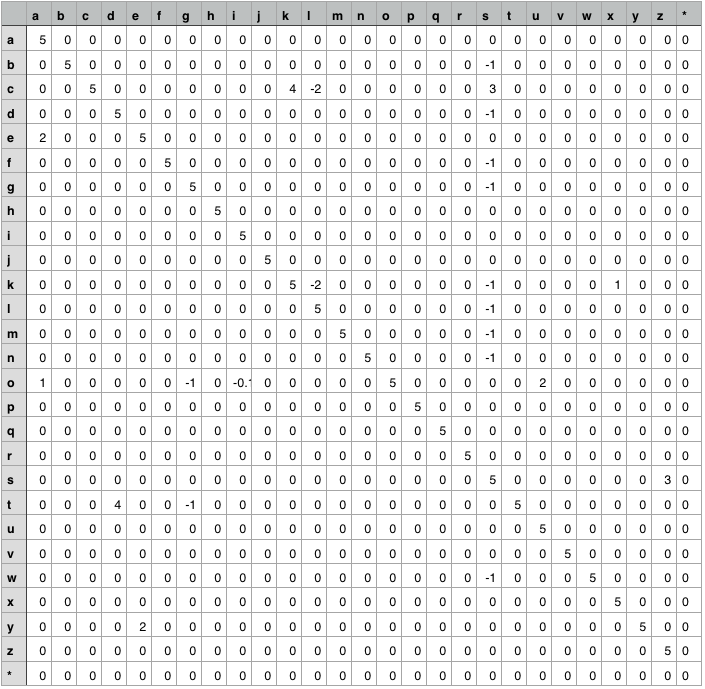
\includegraphics[width=0.5\textwidth]{viterbi_matrix.png}
\subsection*{A-3 Abbreviations: phrases}
\begin{verbatim}
omg	oh my god
idk	I don't know
idek	I don't even know
omfg	oh my fucking god
wtf	what the fuck
smh	shaking my head
ily	I love you
ilysm	I love you so much
tbh	to be honest
idc	I don't care
stfu	shut the fuck up
btw	by the way
ik	I know
idgaf	I don't give a fuck
jk	just kidding
hmu	hit me up
bff	best friend
nvm	never mind
ffs	for fucks sake
oomf	one of my friends
\end{verbatim}
\subsection*{A-4 Text correction example}
\lstset{basicstyle=\footnotesize\ttfamily, 
	tabsize=2,
	backgroundcolor=\color{lightgray},
	showstringspaces=false,
	breaklines=true
}
\begin{lstlisting}
Today stats: No new followers, One unfollower via http://t.co/KQMxmRhDsX
today starts: no new followers, one unfollowers via [url]
why doesn't accio exist in real life this is important
why doesn't action exist in real life this is important
I c ur picture ... but is that really you ??
i see your picture ... but is that really you ??
Straight a synoptic grateful dead towards strange circulating medium displacement: AuoZkEvxf
straight a sympathetic grateful dead towards strange circulating medium displacement: akgfjkdadutdfhsdfkfajf
Im Yeva and I eat poop
im yea and i eat poop
RT @Officialsimyai: If I have to beg fo yo attention den I don't want it 👋🙅💁
if i have to beg for you attention den i don't want it 👋🙅💁
@carinaa888 exactly!! sooo shut ur ass up lol
[username] exactly!! so shut your ass up [laughter]
“@YungJadeTheGawd: I wanna have a cookout tomorrow .” In dere like swimwear“
[username]: i wanna have a cookout tomorrow .” in there like swimwear
RT @natalieben: Greens have got far more votes per minute of TV time than any other party.  #VoteGreen2014. #EP2014
greens have got far more votes per minute of tv time than any other party.  #votegreen2014. #ep2014
We all could die tonight
we all could die tonight
Back 2 Good
back 2 good
one person followed me // automatically checked by http://t.co/XTToHqv7gF
one person followed me // automatically checked by [url]
Why people be mad when someone runs to there ex? No reason for you tryna be a rebound anyway tf lol
why people be mad when someone runs to there ex? no reason for you tryna be a rebound anyway what the fuck [laughter]
RT @BestVinesEver: To a piano tho?! https://t.co/ISSmUHov2Q
to a piano tho?! [url]
RT @TheBucktList: Need it now.🌴 http://t.co/PDXYKSKxfK
need it now.🌴 [url]
@MikeyPosod hell yeah👌haha
[username] hell yeah👌[laughter]
i get high off our memories
i get high off our memories
RT @CourtMitchell17: I feel like power dressing shouldnt be dressing like a man it should be owning our feminity &amp;wearing it proudly. I lov…
i feel like power dressing shouldn't be dressing like a man it should be owning our feminist &amp;wearing it proudly. i love…
Learn About Mountain Climbing from Novice to Experts  http://t.co/oky5Qsf1Df
learn about mountain climbing from notice to experts  [url]
@jdhowa2 Tuesday I typed "Waze is taking me the rapey way so if I'm not there in 10, let's hope my body shuts this whole thing down."
[username] tuesday i typed "wake is taking me the rape way so if i'm not there in 10, let's hope my body shuts this whole thing down."
Slim my new header 💕💕💕 she so fine man 😫😍
slim my new header 💕💕💕 she so fine man 😫😍
FOLLOW ME BÆ @JackDail 66
follow me beÆ [username] 66
@FotMound Can you give examples of a tightly focused theme? #fantasychat
[username] can you give examples of a tightly focused theme? #fantasychat
In love memory daddy http://t.co/OhBTgBZdP3
in love memory daddy [url]
My first jet lag...
my first jet lag...
RT @Nikaxo__: FUCK YALL THEY TRY !
fuck y'all they try !
\end{lstlisting}

\subsection*{A-5 Double Metaphone}
\begin{lstlisting}
Double Metaphone Dict(`people'): [`PPL', `']
Inverted Metaphone Dict(`PPL') = [peaple, buble, babble, peoplle, pablooo, pupil, pppl, people, papell, pebble, peopleeee, pueblo, peoople, payable, poeple, bubbly, bubble, peoiple, bible, bpl, bubbaloo, piebbal, peopl, peopleee, people, bypoll, pablo, bhopal, papal, paypal, peoplee, bobble, peple]
\end{lstlisting}

\lstset{basicstyle=\footnotesize\ttfamily, 
	tabsize=2,
	language=Python,
	backgroundcolor=\color{lightgray},
	commentstyle=\color{mygreen},
	keywordstyle=\color{blue},
	stringstyle=\color{red}\ttfamily,
	showstringspaces=false,
	breaklines=true
}

\section*{References}

\end{document}